\documentclass[letterpaper, 10pt, conference]{IEEEtran}

\usepackage[top=0.75in,bottom=0.75in,right=0.75in,left=0.75in]{geometry}
\IEEEoverridecommandlockouts
\overrideIEEEmargins
\usepackage{graphicx}
\usepackage[utf8]{inputenc}
\usepackage[T1]{fontenc}
\usepackage[polutonikogreek,english]{babel}
\usepackage{fixltx2e}
\usepackage{gensymb}
\usepackage{mathtools}
\usepackage{amssymb}
\usepackage{amsmath}
\usepackage{algorithm}
\usepackage[noend]{algpseudocode}
%\usepackage[font=small]{caption}
%\usepackage{caption}
%\usepackage{subcaption
%\usepackage{booktabs}


\DeclarePairedDelimiter\abs{\lvert}{\rvert}%
\DeclarePairedDelimiter\norm{\lVert}{\rVert}
\newcommand{\greek}[1]{{\selectlanguage{polutonikogreek}#1}}
\newcommand\scalemath[2]{\scalebox{#1}{\mbox{\ensuremath{\displaystyle #2}}}}
\renewcommand{\vec}[1]{\mathbf{#1}}
\hyphenation{op-tical net-works semi-conduc-tor}

\begin{document}
\bstctlcite{IEEEexample:BSTcontrol}

\title{Model Predictive Control for\\Underwater Robots in Ocean Waves}

\author{\IEEEauthorblockN{Daniel Fernández and Geoffrey A. Hollinger}
\IEEEauthorblockA{Robotics Program\\
School of Mechanical, Industrial and Manufacturing Engineering\\
Oregon State University\\
Corvallis, Oregon 97331--6001\\
fernanda@oregonstate.edu, geoff.hollinger@oregonstate.edu}
}

% make the title area
\maketitle
\thispagestyle{empty}
\pagestyle{empty}

\begin{abstract}
%\boldmath
Autonomous marine vehicle decision making is an active avenue of research in the Field Robotics Community. Much of this work includes advancing underwater path planning, localization, and perception. Developments in this field can lead to cost-effective methods of deploying marine energy arrays. The purpose of this document is to summarize some of the more promising research applications as well as justify the use of autonomy in the offshore community. Lorem ipsum dolor sit amet, consectetur adipiscing elit. Duis suscipit, metus a dapibus bibendum, massa est eleifend ligula, egestas tempor risus ante vel lorem. Lorem ipsum dolor sit amet, consectetur adipiscing elit. Nulla vitae orci ac ipsum volutpat lacinia. Fusce tempus sapien nec tempus tincidunt. Phasellus fringilla facilisis sodales. In aliquam velit quam, id pretium metus scelerisque vitae. Maecenas non mollis ante. Vestibulum pretium sed ipsum a aliquam. Cras id pharetra urna, non semper ex. In at nunc at dolor viverra gravida eu iaculis metus. Fusce bibendum, est non porta pellentesque, elit urna porta lacus, vel viverra purus urna eu nibh. Quisque a elementum ipsum, quis iaculis lacus. Ut dictum vestibulum enim sed interdum. Vivamus cursus dui nec est fringilla, nec dignissim sem congue.
\end{abstract}

\begin{IEEEkeywords}	
TBD, marine robotics, wave energy, autonomous path planning, perception, oceanographic monitoring, SLAM, AUV, ROV
\end{IEEEkeywords}

\section{Introduction} 
\label{sec:introduction}

In the intermediate depths of the coastal ocean, the area of ocean bounded by the shoreline and the 200~m isobath \cite{phillips}, wave forces are felt throughout the majority of the water column. Wave motion decays exponentially from the water surface, meaning an object at a sufficient enough depth would not be notably disturbed \cite{D&D}. Because of this decay, as well as their cyclic nature, wave forces are often times neglected in robotic path planning. In field applications where there is a low operational depth, a persistent wave climate, and strict localization constraints, this assumption can quickly break down, resulting in hindered robotic observations. Traditional PID control techniques can be used, but given the periodicity of waves, feedforward techniques should be explored. This paper will outline how Model Predictive Control (MPC) can reduce an underwater robot's position error when station-keeping under the influence of ocean waves.

Implementing MPC requires a prediction horizon where future vehicle states can be determined given a set of associated control actions \cite{camacho}. Next, these future states must be compared with a global minimizing cost function, which in this case is the squared distance from the desired and predicted states. By thresholding the control actions within the minimization function, the need for tuning gains, such as in PID control, is removed \cite{rawlings}. The number of steps that the horizon estimates forward is a variable; however, as it should not be too short or too long. Too little time will not allow for the full dynamics of the system to be accounted for while too much time will be computationally intensive.

The method outlined in this paper applies MPC to underwater station-keeping in a shallow water bathymetry under the influence of a strong sea swell. The calculated control actions are optimized to actuate an underwater robot's thrusters in an anticipatory fashion so that the net result is that the vehicle remains stationary as the waves pass over it. The motivation behind such work is increasing the quality of robotic observations in shallow ocean water as well as reducing the risk of equipment damage while deployed.

The remainder of this paper is organized as follows: the MPC method is further described in section \ref{sec:mpc} and section \ref{sec:waves} describes the wave mechanics used as inputs. Section \ref{sec:dynamics} details the vehicle modeled and overall system dynamics. Section \ref{sec:sim} details the algorithm structure and controller specifics. Section \ref{sec:results} details results of determining optimal horizons, and system performance against a simulated wave field with noisy observations. Finally, concluding remarks are provided in Section \ref{sec:conclusion}. %Figure \ref{fig:structure} shows the paper outline in more detail. 

\section{Model Predictive Control} 
\label{sec:mpc}

The term MPC does not refer to a specific strategy, but a variety of methods which all in some way incorporate the following \cite{camacho}:
\begin{itemize}
  \itemsep0.25em
  \item Modeled state estimator along some time horizon
  \item Cost function to minimize a control sequence 
  \item Receded horizon as optimized control is carried out 
\end{itemize}

MPC requires a model of the system dynamics which can estimate future states given a current state and set of control inputs along a time horizon. The model in this case will include the vehicle dynamics and thruster forces, along with a disturbance matrix to model the wave disturbances on the system. The time horizon is a tuned parameter where larger values give more optimal trajectories at the expense of computation time. 

The sequence of input control actions to the state estimator is optimized by way of a minimizing cost function. Cost functions can be formulated by balancing one or several metrics, i.e. mission duration, energy consumption, or number of sampled observations \cite{lavalle, binney}. Given the station-keeping task, the cost function employed in this work is the sum of squared distances from the desired and predicted states over the current horizon, or:
\begin{equation}
\vec{J} = \sum_{k}^{nSteps}(\vec{\Upsilon}_{target} - \vec{\Upsilon}_k)^2,
\label{eqn1}
\end{equation}
where $nSteps$ is horizon length, $k$ is the current time step in the $nSteps$ horizon, $\vec{\Upsilon}_{target}$ is the desired state, $\vec{\Upsilon}_k$ is the state at time $k$, and $\vec{J}$ is the overall cost to be minimized. 

The control actions are then optimized by comparing the derivatives of the cost with respect to the control actions taken. This Jacobian value is the rate of change of cost per change in control and is minimized as the optimal control action is approached. At each optimization step, the set of control actions is perturbed by the Jacobian and its effects are estimated along the horizon. This is repeated until a set of control actions which minimizes the sum of squares cost function is calculated. This method of cost evaluation and optimization is similar to that used by Medagoda et al in \cite{medagodaMPC}.

\section{Wave Mechanics} 
\label{sec:waves}

According to Linear Wave Theory (LWT), a wave field in a random sea is composed of a superposition of sinusoids. Once decomposed, each sinusoid can then be analyzed as a single monochromatic wave with unique period (T), amplitude (a), and phase offset ($\phi$) \cite{D&D,phillips}. For reference, this paper will instead use the term waveheight (H), which is simply twice the amplitude (H = 2a). In practice, LWT has not just the advantage of ease of implementation, but it has also shown to produce surprisingly accurate results \cite{D&D}. Thus, LWT is often employed as a reliable primary analysis before other nonlinear theories and forms the wave action model used in this paper.

Beneath each component monochromatic wave, wave-induced particle displacements occur in a cyclical fashion. These displacements follow circular paths in deep water waves (d > L/2), and become elliptical as water depth decreases until they are nearly horizontal in the surf zone \cite{D&D}. Associated particle velocities and accelerations can be derived from these trajectories. As stated earlier, the magnitude of these velocities and accelerations decay exponentially through the water column such that they are neglible (< 0.04\%) at a depth equalling approximately half of the surface wavelength (d = L/2) \cite{D&D}. The per-wave, at-depth solutions to these velocity and acceleration equations are used as the primary inputs to the modeled system dynamics.

A field of random sea waves can be decomposed to its component frequency spectra, not unlike an electrical signal, by way of a Fourier Analysis \cite{goda}. blah blah blah Cite \cite{falnes} and \cite{ling}. In this work, the inputted wave field is assumed to be provided to the vehicle as an array of wave period, wave height, and phase offset (T, H, $\phi$). 

\begin{figure}
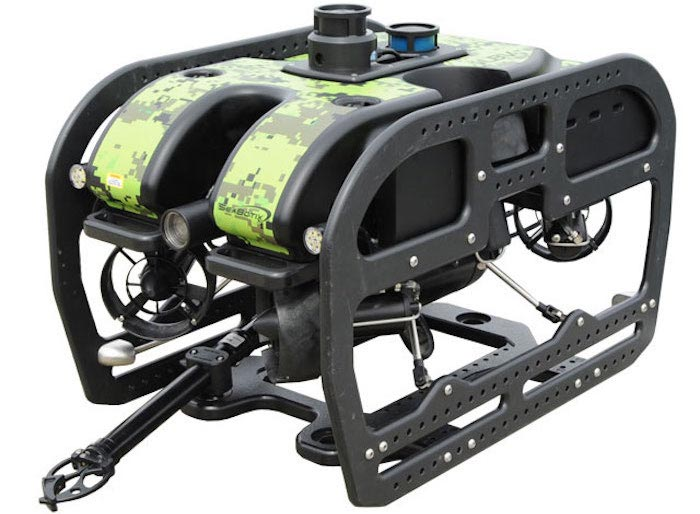
\includegraphics[width=1\columnwidth]{seabotix}
\centering
\caption{A SeaBotix vLBV300 ROV similar to the one modeled in this work. The vehicle has six angled thrusters which control it along five degrees of freedom: heave, sway, surge, roll, and yaw.}
\centering
\label{fig:seabotix}
\end{figure}

\begin{table}
\caption{Vehicle parameters used in simulation}
\begin{center}
\def\arraystretch{1.1}%
\begin{tabular}{ |l|l|l| } 
 \hline 
 Parameter & Symbol & Value \\ 
 \hline
 Density of Seawater & $\rho_{sea}$ & 1030~kg/$m^3$ \\ 
 Incident Area, $\vec{x}$ & $A_{i,\vec{x}}$ & xxx \\ 
 Incident Area, $\vec{z}$ & $A_{i,\vec{z}}$ & xxx \\
 Moment of Inertia, $\vec{x}$ & $I_{xx}$ & xxx \\
 Moment of Inertia, $\vec{z}$ & $I_{zz}$ & xxx \\
 Dry Mass & $m_{dry}$ & 22.2~kg \\
 Added Mass, $\vec{x}$ & $m_{add,x}$ & 8.1~kg \\
 Added Mass, $\vec{z}$ & $m_{add,z}$ & 36.7~kg \\
 Drag Coefficient, $\vec{x}$ & $c_{d,x}$ & 0.84\\
 Drag Coefficent, $\vec{z}$ & $c_{d,z}$ & 1.06\\
 Max Thruster Force & $T_{max}$ & 29.7~N \\
 Thruster Angle, Forward & $\theta_f$ & 35\degree \\
 Thruster Angle, Aft & $\theta_a$ & 45\degree \\
 Thruster Angle, Vertical & $\theta_v$ & 20\degree \\
 \hline
\end{tabular}
\end{center}
\label{table:vehicleData}
\end{table}

\section{System Dynamics} 
\label{sec:dynamics}

Underwater vehicles can be classified into one of two generic categories: manned and unmanned vehicles. Unmanned Underwater Vehicles (UUV) are often labeled as synonymous with Autonomous Underwater Vehicles (AUV). This can be misleading as it is not an accepted standard. For the scope of this paper, the term Remotely Operated Vehicle (ROV) will be used to describe a tethered unmanned vehicle whose operation may or may not be tele-operated \cite{ROV}. The ROV modeled for this work is the SeaBotix vLBV300 as shown in Figure \ref{fig:seabotix}. 

\subsection{Vehicle Model}

The SeaBotix vLBV300 ROV has six vectored thrusters controlling motion along five degrees of freedom. For the scope of this work, only the surge and heave directions, or global $\vec{x}$ and $\vec{z}$, will be considered. The vehicle is assumed to be a rigid body, and irrotational in the water flow. Since its size is well below the wavelength, its motion is assumed to follow that of a particle. Vehicle dimensions, mass parameters, and thruster forces are provided in Table \ref{table:vehicleData}. Moment of inertia and center of gravity data is provided by Dassault Systèmes SolidWorks. Added mass values are provided from Ansys AQWA. Drag coefficient data is provided by the manufacturer. The differential equations defining the ROV motion is: 
\begin{equation}
\vec{M}\dot{\vec{v}}_a + \vec{F}_d + \vec{F}_g + \vec{F}_c = \vec{F}_{thrust},
\label{eqn2}
\end{equation}
where $\vec{M}$ is a mass term containing the dry and added masses, $m_{dry}$ and $m_{add}$, $\vec{v}_a$ is the absolute velocity of the vehicle with respect to the inertial reference frame, $\vec{F}_d$ is the drag force from the water, $\vec{F}_g$ is the force of gravity, $\vec{F}_c$ is the coriolis force, and $\vec{F}_{thrust}$ is the ROV thruster force. By assuming that coriolis force is neglible and that the vehicle is neutrally buoyant, the $\vec{F}_c$ and $\vec{F}_g$ terms drop out. Substituting inertia and drag relations, Equation \ref{eqn2} becomes: 
\begin{equation}
m_{dry} \dot{\vec{v}}_a + m_{add} \dot{\vec{v}}_r  - \frac{1}{2} \rho_{sea} A_i c_d \abs{\dot{\vec{v}}_r} \dot{\vec{v}}_r = \vec{F}_{thrust},
\label{eqn3}
\end{equation}
where $\vec{v}_r$ is the velocity of the vehicle relative to the water, which acts on the added mass term. Substituting heave, surge, and particle velocity components, Equation \ref{eqn3} becomes:
\begin{equation}
\begin{split}
\vec{F}_{thrust} = \begin{bmatrix} m_{dry}+m_{add,\vec{x}} \\ m_{dry}+m_{add,\vec{z}} \end{bmatrix} \begin{bmatrix} \ddot{\vec{x}} \\ \ddot{\vec{z}} \end{bmatrix} - \begin{bmatrix} m_{add,\vec{x}} \\ m_{add,\vec{z}} \end{bmatrix} \begin{bmatrix} \dot{\vec{v}}_{p,\vec{x}} \\ \dot{\vec{v}}_{p,\vec{z}} \end{bmatrix} \\- \frac{\rho_{sea}}{2} \begin{bmatrix} A_{i,\vec{x}}C_{d,\vec{x}} \\ A_{i,\vec{z}}C_{d,\vec{z}} \end{bmatrix} \begin{bmatrix} \abs{\dot{\vec{x}}-\vec{v}_{p,\vec{x}}} (\dot{\vec{x}}-\vec{v}_{p,\vec{x}}) \\ \abs{\dot{\vec{z}}-\vec{v}_{p,\vec{z}}} (\dot{\vec{z}}-\vec{v}_{p,\vec{z}}) \end{bmatrix},
\label{eqn4}
\end{split}
\end{equation}
where $\vec{v}_p$ is the particle velocity at a time and position beneath a monochromatic wave. For added reference, $\vec{v}_a$ = $\vec{v}_r$ + $\vec{v}_p$, and $\dot{\vec{v}}_{a,\vec{x}}$ = $\ddot{\vec{x}}$, $\dot{\vec{v}}_{a,\vec{z}}$ = $\ddot{\vec{z}}$.

\subsection{State Space Form}

The differential equations are now rewritten in state space form solvable by the simulator. This takes the form:
\begin{equation}
\dot{\vec{\Upsilon}} = \begin{bmatrix} \dot{\vec{x}} & \ddot{\vec{x}} & \dot{\vec{z}} & \ddot{\vec{z}}\end{bmatrix}^T = \vec{A}\vec{x} + \vec{B}\vec{u} + \vec{D},
\label{eqn5}
\end{equation}
where
\begin{equation}
\vec{A}\vec{x} = \begin{bmatrix} 0 & 1 & 0 & 0 \\ 0 & 0 & 0 & 0 \\ 0 & 0 & 0 & 1 \\ 0 & 0 & 0 & 0  \end{bmatrix} \begin{bmatrix} \vec{x} \\ \dot{\vec{x}} \\ \vec{z} \\ \dot{\vec{z}} \end{bmatrix},
\label{eqn6}
\end{equation}
\begin{equation} 
\vec{B}\vec{u} = \scalemath{0.69}{ \frac{T_{max}}{m_{dry}} \begin{bmatrix} 0 & 0 & 0 & 0 & 0 & 0 \\ cos\theta_f & cos\theta_f & -cos\theta_a & -cos\theta_a & 0 & 0 \\ 0 & 0 & 0 & 0 & 0 & 0 \\ 0 & 0 & 0 & 0 & -cos\theta_v & -cos\theta_v \end{bmatrix} \begin{bmatrix} u_1 \\ u_2 \\ u_3 \\ u_4 \\ u_5 \\ u_6 \end{bmatrix} },
\label{eqn7}
\end{equation}
and
\begin{equation} 
\vec{D} = \begin{bmatrix} 0 \\ \frac{\dot{\vec{v}}_{p,\vec{x}}}{m_{dry}} + \frac{\rho_{sea} A_{i,\vec{x}} C_{d,\vec{x}}}{2(m_{dry}+m_{add,\vec{x}})} \abs{\dot{\vec{x}}-\vec{v}_{p,\vec{x}}} (\dot{\vec{x}}-\vec{v}_{p,\vec{x}})  \\ 0 \\ \frac{\dot{\vec{v}}_{p,\vec{z}}}{m_{dry}} + \frac{\rho_{sea} A_{i,\vec{x}} C_{d,\vec{z}}}{2(m_{dry}+m_{add,\vec{z}})} \abs{\dot{\vec{z}}-\vec{v}_{p,\vec{z}}} (\dot{\vec{z}}-\vec{v}_{p,\vec{z}}) \end{bmatrix}. 
\label{eqn8}
\end{equation}

The $\vec{u}$ vector in Equation \ref{eqn7} refers to motor inputs to each of the vehicle's six vectored thrusters. $\vec{u}_1$ and $\vec{u}_2$ are the forward thrusters, $\vec{u}_3$ and $\vec{u}_4$ are the aft thrusters, and $\vec{u}_5$ and $\vec{u}_6$ are the vertical thrusters.

\section{Simulator Setup}
\label{sec:sim}

The ROV was simulated along a 240-s long time vector with 0.2~s discretizations. All robot thruster actuations and wave disturbances occur along the global $\vec{x}$ and $\vec{z}$ axes. Each motor input simulated by the $\vec{B}\vec{u}$ matrix in Equation \ref{eqn7} is a thresholded value between [-1,1], which correlates to a percentage of maximum possible thrust. All forward-looking state estimations and robot movements use the MATLAB function \Call{ode45}{} which uses a variable step Runge-Kutta Method to numerically solve the system differential equations \cite{ode45}.

\subsection{Wave Field Model} 

The bathymetry and wave climate selected for analysis is similar to that of the National Northwest Marine Renewable Energy Center (NNMREC) North Energy Test Site (NETS) in the coastal Pacific Ocean two nautical miles out of Newport, Oregon \cite{ling}. The operational depth at NETS is approximately 50~m. The wave field used by the simulator is a set of eight different periods, heights, and phases (T, H, $\phi$) and is detailed in Table \ref{table:waveData}. Because of the 2 dimensional analysis along only surge and heave motions, wave angles are set to 0.

\begin{table}
\caption{Wave field parameters used in simulation}
\begin{center}
\def\arraystretch{1.1}%
\begin{tabular}{ |l|c|c|c|c|c|c|c|c|c| } 
 \hline 
 Component Wave & 1 & 2 & 3 & 4 & 5 & 6 & 7 & 8 \\ 
 \hline
 Wave Period, s & 10 & 8 & 12 & 11 & 6 & 7 & 9 & 25  \\ 
 Wave Height, m & 1.8 & 0.9 & 1.6 & 1.3 & 0.4 & 0.5 & 1.1 & 0.7 \\ 
 Phase, radians & -$\frac{\pi}{2}$ & -$\frac{\pi}{4}$ & -$\frac{5\pi}{8}$ & $\frac{4\pi}{13}$ & -$\frac{\pi}{15}$ & $\frac{\pi}{3}$ & -$\frac{\pi}{18}$ & -$\frac{7\pi}{4}$\\
 \hline
\end{tabular}
\end{center}
\label{table:waveData}
\end{table}

Component wavelengths (L), wave numbers (k), and frequencies ($\omega$) are solved for by way of the dispersion relation \cite{D&D}. The superimposed wave field shown in Figure \ref{fig:eta} is then constructed by the water surface wave equation shown below:  
\begin{equation} 
\eta = \frac{H}{2}cos(k\vec{x}-\omega\vec{t}+\phi) .
\label{eqn9}
\end{equation}

\begin{figure}
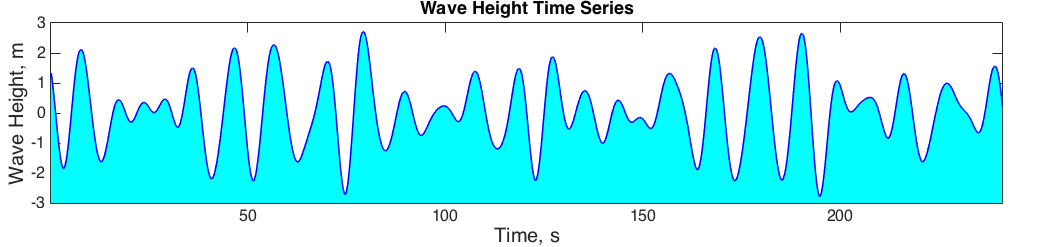
\includegraphics[width=1\columnwidth]{eta}
\vspace*{-14pt}
\centering
\caption{A time series of the wave profile over the 240~s simulated time constructed using the parameters listed in Table \ref{table:waveData}.}
\label{fig:eta}
\end{figure}

Prior to any forward state estimation or any simulated vehicle motion, the wave action, or particle accelerations and velocities, are calculated for the robot's current position in time and space. These accelerations and velocities are calculated for each wave and summed using the superposition principle in the function \Call{getParticles}{} shown in Algorithm \ref{alg:MPC}.

\subsection{Algorithm Layout}

The \Call{MPC}{} algorithm shown in Algorithm \ref{alg:MPC} requires four inputs. The first, $t$, is a time object containing the overall time vector and horizon and discretization parameters. The second input, $\lambda$, is an object containing all relevant wave spectra data. The third input is the robot object, which contains the vehicle dynamics, states, and error history. This object is often passed as an input to support functions and returned with a modified state. The last input, $\Upsilon_{target}$, is the target state.

\begin{algorithm}
\caption[caption]{MPC for Ocean Wave Station Keeping \hspace{\textwidth}where $t$ is a vector of time, $\lambda$ is an object containing all relevant wave spectra data, and $\Upsilon$ represents states in time and space.}
\label{alg:MPC}
\begin{algorithmic}[1]

\Procedure{$MPC$}{ robot } \Comment{Inputs: $t$, robot, $\lambda$, $\Upsilon_{target}$}
\State $n\gets1$
\State $\eta \gets$ \Call{loadSeaState}{ $t$, $\lambda$, $\Upsilon_{initial}$ }
\While{$n<$ simulatorOff}
\State input $\gets$ \Call{getForecast}{ $t$, robot, $\lambda$, $\Upsilon_{target}$, $n$ } 
\State robot $\gets$ \Call{moveRobot}{ $t$, robot, $\lambda$, input, $n$ } 
\State $n \gets n+1$
\EndWhile
\EndProcedure

\Function{getForecast}{ $t,$ robot, $\lambda, \Upsilon_{target}, count$ }
\State $i \gets 1$
\State $nSteps \gets t.Horizon$ / $t.Discretization$
\State $J_i$, $u_i$, $\Upsilon_i \gets$ \Call{initializeInput}{ robot }
\State $\delta \gets$ \Call{initializeDelta}{ } 
\While{$i$ < maxIterations \textbf{and} $\delta$ > exitCriteria}
\State $u_{i+1} \gets u_{i} - \delta$
\For {$k\in [1,2,...,nSteps]$}
\State $\vec{v}_p, \dot{\vec{v}}_p \gets$ \Call{getParticles}{ $t$, $\Upsilon_i(k)$, $\lambda$ }
\State $\Lambda \gets \vec{v}_p, \dot{\vec{v}}_p$
\State $\Upsilon_{i+1}(k) \gets$ \Call{getState}{ $t$, robot, $\Lambda$, $u_{n+1}(k)$ }
\State $J_{i+1}(k) \gets$ \Call{getCost}{ $\Upsilon_{target}$, $\Upsilon_{i+1}(k)$ }
\EndFor
\State $\delta \gets$ \Call{getJacobian}{ $J_i$, $J_{i+1}$, $u_i$, $u_{i+1}$ }
\State $u_i \gets u_{i+1}$
\State $J_i \gets J_{i+1}$
\State $\Upsilon_i \gets \Upsilon_{i+1}$
\State $i \gets i+1$
\EndWhile
\State \Return $u_{i+1}$
\EndFunction

\end{algorithmic}
\end{algorithm}

Once all inputs are passed through, \Call{MPC}{} runs by first generating the initial sea state at \Call{loadSeaState}{} from the wave spectra data in $\lambda$. Then, and until some cessation criteria, \Call{getForecast}{} generates the optimized motor inputs for each thruster while \Call{moveRobot}{} passes those inputs and moves the robot one step forward along that control vector. 

\Call{getForecast}{} is further detailed in the algorithm description. Here, the function \Call{initializeInputs}{} generates initial cost, control, and state vectors, or $J_i$, $u_i$, and $\Upsilon_i$ respectively. The initial control vector, $u_i$, is a set of PD control actions along the $nSteps$ horizon. \Call{initializeDelta}{} creates a value, $\delta$, to perturb $u_i$. In the body of the following for statement, this perturbation generates a new input, $u_{i+1}$, and is then evaluated. First, the wave forces along its trajectory, $\vec{v}_p$ and $\dot{\vec{v}}_p$, are calulated through \Call{getParticles}{}. Next, $\vec{v}_p$, $\dot{\vec{v}}_p$, and the control vector, $u_{i+1}$ are passed in to \Call{getState}{} which estimates the resulting predicted state, $\Upsilon_{i+1}$. Last, $\Upsilon_{i+1}$ is evaluated with respect to the target state, $\Upsilon_{target}$ in \Call{getCost}{} by way of the cost function in Equation \ref{eqn1}.

After the cost, $J_{i+1}$, is evaluated over the entire $nSteps$ horizon, the function \Call{getJacobian}{} evaluates the Jacobian, or $\delta \vec{J} / \delta \vec{u}$, and returns a new $\delta$ value. This value translates the rate at which cost changes to a change in control inputs, and a $\delta$ value growing smaller implies that a control vector is nearing optimal.  At the end of each evaluation, if $\delta$ does not meet some $exitCriteria$, a new input vector is generated and the process is repeated. If it does; however, the optimized input vector, $u_{i+1}$, is returned and the robot moves forward along that trajectory. 

\section{Results} 
\label{sec:results}

One challenge when implementing MPC is determining the optimal prediction horizon. Section \ref{results:optimal} details how an optimal horizon which balances solution accuracy with computation time is selected for this work. Section \ref{results:perform} evaluates the optimal prediction horizon controller against a standard PD controller in the same wave climate. Finally, in section \ref{results:noise}, the same optimal trajectory is compared with a PD controller with simulated sensor noise. For these simulations, the robot was to maintain a depth of $\vec{z}$ = -15~m below the surface, or $\Upsilon_{target}$ = [0, -15]. Though the simulator is designed to simulate any depth in the 50~m bathymetry, simulations were not run at multiple depths as the results would have been scaled throughout. Also, the $exitCriteria$ for an optimized trajectory was set to 5~mm. 

\subsection{Determination of Optimal Horizon} \label{results:optimal}

An optimal prediction horizon for MPC should reasonably balance computation time against position error. This is a discretionary characteristic as certain implementations may have stricter tolerances. In this approach, Simulations were run with a range of horizons from 0.2~s to 3.0~s. Table \ref{table:optimalHorizon} shows total errors and computation times per horizon. 

\begin{table}[h]
\caption{Performance of various simulated horizons}
\begin{center}
\def\arraystretch{1.1}%
\begin{tabular}{ |l|c|c|c|c|c|c|c| } 
 \hline 
 Horizon Time, s & 0.2 & 0.4 & 0.8 & 1.0 & 1.6 & 2.0 & 3.0 \\ 
 \hline
 $\Sigma$ Position Error, m & xxx & xxx & xxx & xxx & xxx & xxx & xxx \\ 
 $\Sigma$ Computation Time, s & xxx & xxx & xxx & xxx & xxx & xxx & xxx \\ 
 Comparison Metric & xxx & xxx & xxx & xxx & xxx & xxx & xxx\\
 \hline
\end{tabular}
\end{center}
\label{table:optimalHorizon}
\end{table}

Based on the information in Table \ref{table:optimalHorizon}, the optimal horizon is xx. Of note is the significantly less-than-optimal results from the shorter horizon controllers. This is likely due to an induced "nearsightedness" where the limited horizon does not allow for the robot to take proper advantage of the wave dynamics as a longer horizon would do. 

\subsection{Optimal Horizon Controller Performance} \label{results:perform}

Another set of simulations is run where the robot employs MPC with the determined optimal horizon. The optimized trajectory position error is compared with that of a robot using a traditional PD controller under the influence of the same wave field. A free-floating, non-actuated robot disturbed by the same waves is simulated as well for reference. Table \ref{table:errorSum} shows the summed error over these simulations and Figure \ref{fig:errorComp} details the positional errors for the PD and MPC controllers over the length of the time vector.

\begin{figure*}
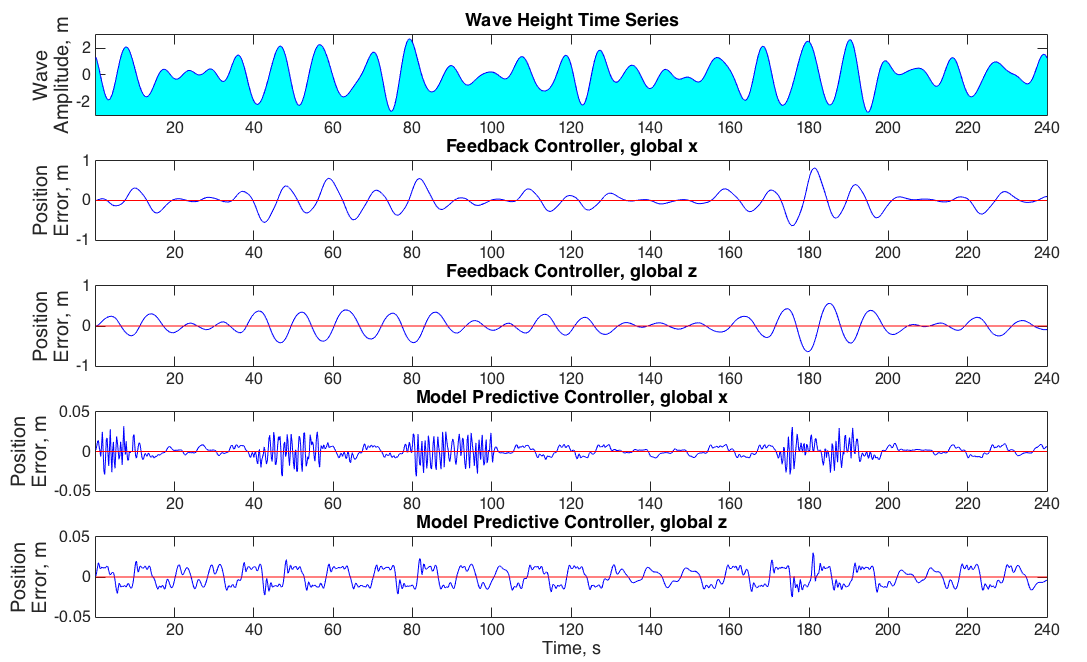
\includegraphics[width=1\linewidth]{compFig2}
%\vspace*{-14pt}
\centering
\caption{Position errors in global $\vec{x}$ and $\vec{z}$ coordinates when comparing a traditional feedback controller with a model predictive controller. As shown, MPC returns error values one order of magnitude lower than PD Control. Summed error values for these results are shown in Table \ref{table:errorSum}.} 
\label{fig:errorComp}
\end{figure*}

\begin{table}[h]
\caption{MPC Performance Comparison}
\begin{center}
\def\arraystretch{1.1}%
\begin{tabular}{ |l|c|c| } 
 \hline 
  & $\Sigma error_\vec{x}$, m & $\Sigma error_\vec{z}$, m \\ 
 \hline
 Model Predictive Control & 7.41 & 11.47 \\ 
 PD (Feedback) Control & 190.24 & 191.22 \\ 
 No Control (drift) & 1225.08 & 1151.53 \\
 \hline
\end{tabular}
\end{center}
\label{table:errorSum}
\end{table}

As shown here, the MPC does this and that and that and this. The PD does not however, as it does that and this before doing this and that. In Figure \ref{fig:errorComp}, the wave field time series is provided to show the correlation between wave height, H, which is directly proportional with wave forces in the water column \cite{D&D}, and position error below the waves. 

\subsection{Sensor Noise Impact} \label{results:noise}

Simulations were then carried out to compare optimized trajectories to the effects of simulated sensor observation noise. For this simulation set, Gaussian noise is injected to the vehicle's perceived value of wave height, H. The H parameter was selected instead of other forms of localization noise because of the specific vehicle's sensor payload. The Inertial Measurement Unit (IMU) has less resolution than the Doppler Velocity Log (DVL). It is thus more likely that the IMU would give inaccurate observations on the pressure field above it (the wave action) than the DVL would on vehicle localization. Obviously, this assumes the DVL has bottomlock. 

[more on noise setup]\cite{GP}. [more on noise setup] [more on noise setup] [more on noise setup] [more on noise setup] [more on noise setup] [more on noise setup] [more on noise setup] [more on noise setup] [more on noise setup] [more on noise setup] [more on noise setup] [more on noise setup]

\begin{table}[h]
\caption{Noisy World Table}
\begin{center}
\def\arraystretch{1.1}%
\begin{tabular}{ |l|c|c| } 
 \hline 
  & heading, m & heading, m \\ 
 \hline
 stuff & xxx & xxx \\ 
 stuff & xxx & xxx \\ 
 more stuff & xxx & xxx \\
 \hline
\end{tabular}
\end{center}
\label{table:noiseData}
\end{table}

As can be seen here, this data is totally accurate and this method is super cool. Its designer is likewise pretty cool too and should probably be allowed to graduate in the immediate future.

\begin{figure}
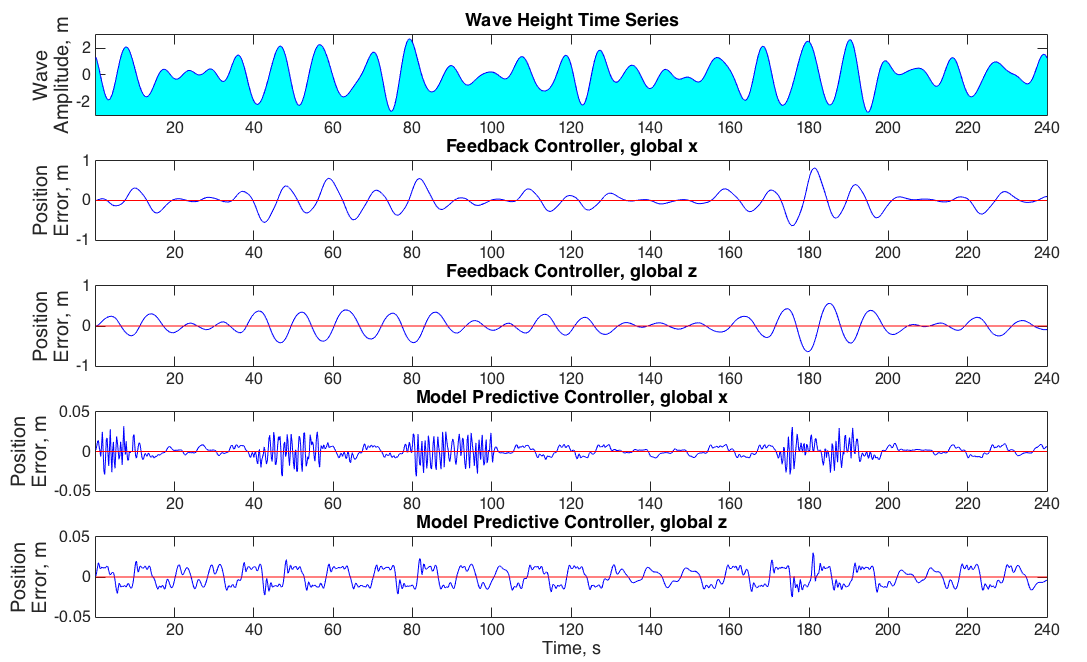
\includegraphics[width=1\linewidth]{compFig2}
%\vspace*{-14pt}
\centering
\caption{THIS DATA IS NO GOOD. This will be a similar structured chart as before except the sensor noise will be incorporated.} 
\label{fig:noiseErrorComp}
\end{figure}

Figure \ref{fig:noiseErrorComp} shows the MPC with noise against the same PD controller as in Section \ref{results:perform}. The simulated IMU sensor noise does not affect the PD controller as it only uses DVL data. [more results talk] [more results talk] [more results talk] [more results talk] [more results talk] [more results talk] [more results talk] [more results talk] [more results talk] [more results talk] [more results talk] [more results talk] [more results talk] [more results talk] [more results talk] [more results talk] [more results talk] [more results talk] [more results talk] [more results talk] [more results talk] [more results talk] [more results talk]

\section{Conclusions and Future Work} 
\label{sec:conclusion}

This paper presented some of the accomplishments in the marine robotic community. These included advancements in autonomous underwater path planning, localization, and perception. Efficient path planning helps reduce overall mission cost and time by optimizing methods of navigating. Localization issues in an environment absent GPS and long range wireless transmissivity prioritize the need for well-developed SLAM techniques with minimal input. Robotic perception in the underwater domain further complicates research efforts. 

These advancements in underwater autonomy will be pivotal in the development of offshore energy arrays, since low-cost robotic platforms inspecting, monitoring, and manipulating infrastructure can reduce deployment costs drastically. Over the course of the NNMREC ALFA project, robust algorithms for these marine platforms to support WEC's will lead to improved scaled economics and further global wave energy development. As more challenges are addressed, this will help secure wave energy extraction as the premier sustainable energy source for the 21st century.

wow! such future work


%\appendices
%\section{HERE WE GO}
% garbage

% use section* for acknowledgement

\section*{Acknowledgments}
This work and other NNMREC ALFA research is supported by Department of Energy DE-EE-0006816.0000.

\ifCLASSOPTIONcaptionsoff
  \newpage
\fi

% trigger a \newpage just before the given reference
% number - used to balance the columns on the last page
% adjust value as needed - may need to be readjusted if
% the document is modified later
%\IEEEtriggeratref{8}
% The "triggered" command can be changed if desired:
%\IEEEtriggercmd{\enlargethispage{-5in}}

\nocite{huynh, geoffadapt, geoffuncertainty, colby, brekken1, brekken2, bosma, ballard, MAS}

\bibliography{main}
\bibliographystyle{IEEEtran}

%\end{main}

%\begin{thebibliography}{1}

%\bibitem{IEEEhowto:kopka}
%H.~Kopka and P.~W. Daly, \emph{A Guide to \LaTeX}, 3rd~ed.\hskip 1em plus
%  0.5em minus 0.4em\relax Harlow, England: Addison-Wesley, 1999.

%\end{thebibliography}

% biography section
% 
% If you have an EPS/PDF photo (graphicx package needed) extra braces are
% needed around the contents of the optional argument to biography to prevent
% the LaTeX parser from getting confused when it sees the complicated
% \includegraphics command within an optional argument. (You could create
% your own custom macro containing the \includegraphics command to make things
% simpler here.)
%\begin{biography}[{\includegraphics[width=1in,height=1.25in,clip,keepaspectratio]{mshell}}]{Michael Shell}
% or if you just want to reserve a space for a photo:

%\begin{IEEEbiography}[{\includegraphics[width=1in,height=1.25in,clip,keepaspectratio]{picture}}]{John Doe}
%\blindtext
%\end{IEEEbiography}

% You can push biographies down or up by placing
% a \vfill before or after them. The appropriate
% use of \vfill depends on what kind of text is
% on the last page and whether or not the columns
% are being equalized.

%\vfill

% Can be used to pull up biographies so that the bottom of the last one
% is flush with the other column.
%\enlargethispage{-5in}




% that's all folks
\end{document}
